\begin{frame}
\frametitle{Large Hadron Collider (LHC)}

\begin{columns}[T] % align columns

\begin{column}{.50\textwidth}
\begin{itemize}
\item A 27km ring of superconducting magnets in a circular tunnel $\sim$100m under the Swiss-French border near Geneva
\item The world's highest energy proton-proton collider (replaced Tevatron at Fermilab for this kind of physics)
\end{itemize}
\end{column}%


\begin{column}{.50\textwidth}
\begin{figure}[htbp]
\begin{center}
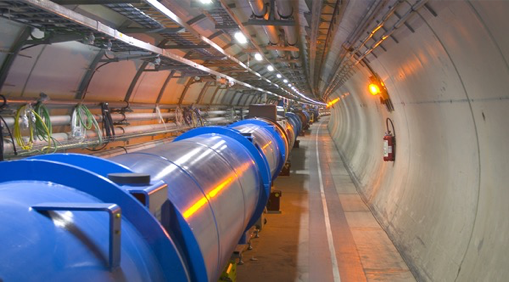
\includegraphics[width=0.9\textwidth]{images/lhc-tunnel.png}
%\caption{}
%\label{fig:example2}
\end{center}
\end{figure}
\end{column}%

\end{columns}

\begin{itemize}
\item From an initial project idea more than 30 years ago, it was built in the existing tunnel designed for previous LEP accelerator
\item The experiments began planning 25 years ago
\end{itemize}


%\small{Example Text}

\end{frame}


